\section{Experimental evaluation}

\subsection{Experiment setup}

\subsubsection{Datasets}

The proposed methods were experimentally verified on several datasets. The datasets Cora and CiteSeer \cite{yang_revisiting_2016} were used with the \enquote{full} train-test split as in \cite{chen_fastgcn_2018}, as well as the Enzymes dataset \cite{morris_tudataset_2020}, where only the 30\todo{check} largest graphs were selected. Two larger datasets were also used, the DBLP dataset \cite{bojchevski_deep_2018} containing 17 716 nodes and 105 734 edges, and the PubMed dataset \cite{yang_revisiting_2016} containing 19 717 nodes and 88 648 edges.

\subsubsection{Methodology of experiments}

The hyper-parameters for both the node2vec model used for the embedding training and the multi-layer perceptron used for downstream classification were initially set to values used in prior art (see \cite{fey_fast_2019, hu_open_2021}) and then manually fine-tuned for each dataset.

For the Cora dataset, the node2vec model generated an embedding into \( \mathfield{R}^{128} \) from \( 4 \) random walks of length \( 20 \) for each node with a context window of size \( 5 \). The optimizer ADAM \cite{kingma_adam:_2017} was used with a learning rate of \( 0.01 \) and batches of \( 128 \) samples. The model was trained for \( 5 \) epochs and in each step of the adaptive prolongation, \( 100 \) nodes were prolonged. The MLP classifier using the embeddings featured \( 3 \) linear layers of \( 128 \) neurons with batch normalization after each layer. Each layer was normalized using dropout \cite{srivastava_dropout_2014} with the rate of \( 0.5 \). Finally, a linear layer was used for the class prediction. ADAM with a learning rate of \( 0.01 \)  was used for \( 30 \) epochs of training with the cross-entropy loss function. Dataset features weren't used for the classifier training as the aim of this work is to compare the embeddings. The experiment was run \( 10 \) times end-to-end and results averaged. For other datasets, the overall design of the experiment was identical, with the only difference being in the values of some hyper-parameters. Additionally, for the Enzymes datasets, the results weren't averaged across multiple runs, but across independent runs over all the graphs instead. The hyper-parameter values for all datasets are listed in Table \ref{tab:hyperparameter-values}. The experiments were implemented using PyTorch \cite{paszke_pytorch_2019} and PyTorch Geometric \cite{fey_fast_2019}.\todo{Dokumentovat, kdy se dělají kroky HARP iterace, kolik jich bylo - tady, nebo níže}

\begin{table}
  \caption{Hyper-parameter values used for different datasets}
  \label{tab:hyperparameter-values}
  \begin{tabular}{lrrrrr}
    \toprule
    Hyper-parameter        & Cora & CiteSeer & Enzymes & PubMed & DBLP \\
    \midrule
    Embedding dimension    & 128  & 32       & 8       & 64     & 32   \\
    \# of random walks     & 4    & 5        & 5       & 3      & 2    \\
    Random walk length     & 20   & 20       & 10      & 40     & 20   \\
    Context window size    & 5    & 5        & 5       & 20     & 5    \\
    Node2vec learning rate & 0.01 & 0.01     & 0.01    & 0.01   & 0.01 \\
    Node2vec batch size    & 128  & 128      & 8       & 128    & 128  \\
    Node2vec epochs        & 5    & 7        & 2       & 1      & 1    \\
    \# of prolonged nodes  & 100  & 150      & 2       & 1000   & 800  \\
    \# of MLP layers       & 3    & 3        & 2       & 1      & 3    \\
    MLP hidden layer width & 128  & 256      & 16      & 128    & 256  \\
    Dropout rate           & 0.5  & 0.5      & 0.5     & 0.5    & 0.5  \\
    MLP learning rate      & 0.01 & 0.01     & 0.01    & 0.01   & 0.01 \\
    MLP epochs             & 30   & 80       & 10      & 300    & 300  \\
    \# of runs             & 10   & 10       & 1       & 10     & 10   \\
    \bottomrule
  \end{tabular}
\end{table}

\subsection{Evaluation of the adaptive approach}

In order to study the effect of the adaptive prolongation, the adaptive prolongation method was used to assess the performance of a downstream classifier at different coarsening levels. A node2vec model as described in the previous Section was trained with adaptive prolongation based on coarsenings pre-computed by HARP coarsening as described in Section \ref{sec:harp-coarsening}. For each prolongation step, the intermediary embedding was afterwards fully prolonged to obtain an embedding of the original graph \( G \). A classifier was then trained with this embedding as input. This setup allows us to compare classification accuracy at each step of the adaptive prolongation. Figure \ref{fig:adaptive-coarsening} shows the results of this experiment, compared with a baseline node2vec model (that is, without any coarsening or prolongation) that was trained for the same number of epochs as the total epochs of the adaptive model over all prolongation steps.

The behaviour of the model somewhat differs between the used datasets. For each dataset, the model starts from a very low performance, which quickly rises as the model trains for several prolongation steps. The model trained on CiteSeer attains performance comparable to the reference model when approximately half of all nodes are available to it.On the other hand, with Cora, the model slowly approaches the reference model over the whole training, only reaching comparable performance at a point where nearly the whole graph is available to it. Models trained on the two larger datasets, DBLP and PubMed, exhibit a categorically different behaviour. Both models reach a local maximum at around 14\% of the graph, followed by a slight decline and gradual approach to the baseline. This suggests a global structure in the data, which the model is learned at the point of the local maxima. Following that, this global structure may be obscured due to noise in the data.\todo{Můžu si tohle dovolit říct?}\todo{Enzymes}

\todo[inline]{Possibly include statistical significance testing.}

\begin{figure}
  \centering
  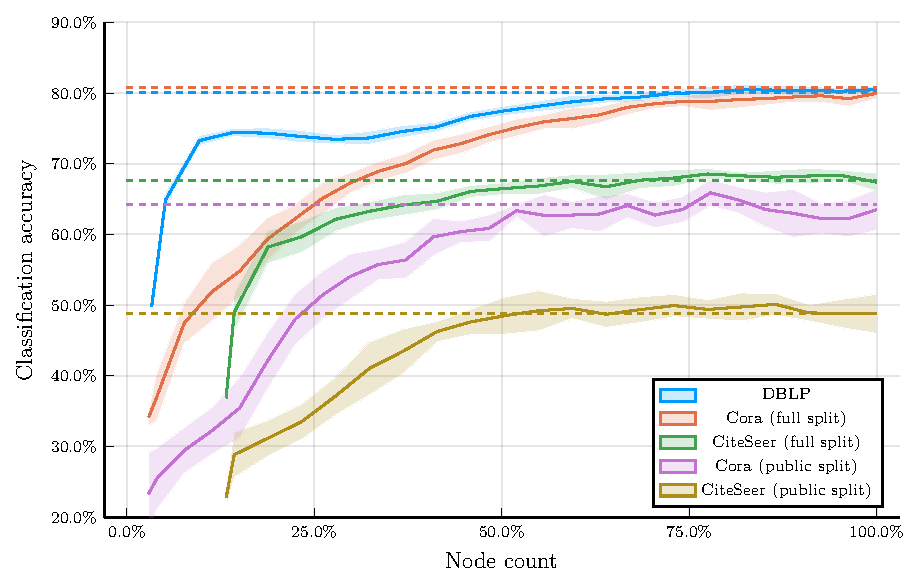
\includegraphics[width = \linewidth]{images/adaptive-coarsening/adaptive-coarsening.pdf}
  \caption{Downstream classifier accuracies at different steps of adaptive prolongation. Dashed line shows the baseline node2vec model accuracy. The node count is taken relative to the total node count in each dataset. The shaded area represents one standard deviation over multiple runs.}
  \label{fig:adaptive-coarsening}
\end{figure}

\subsection{Relation to graph properties}

\todo[inline]{Compare the adaptive coarsening with local graph measures of graph homophilly}

\subsection{Comparison of coarsening approaches}
\todo[inline]{Compare the coarsenings measured by the graphs from previous section}

\begin{figure}
  \centering
  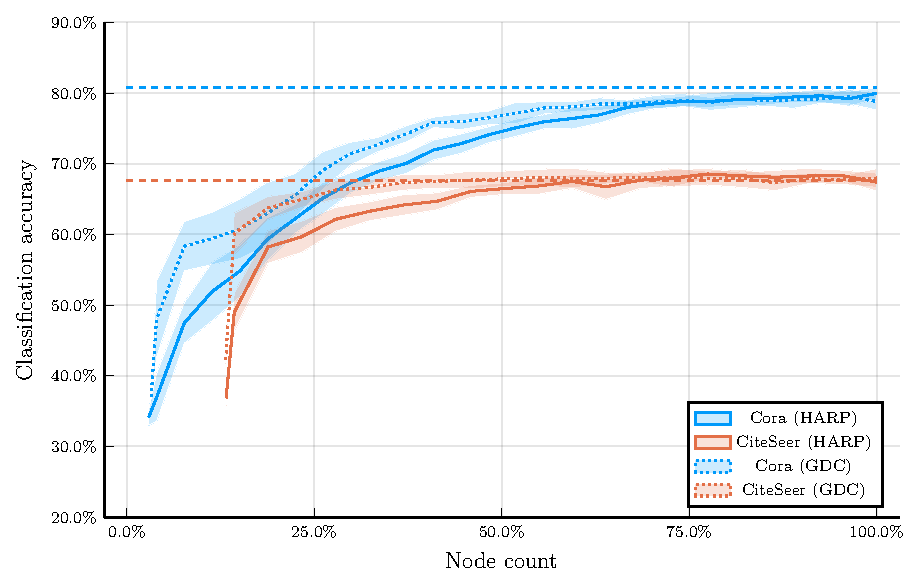
\includegraphics[width=\linewidth]{images/coarsening-algorithms/coarsening-algorithms.pdf}
  \caption{Coarsening algorithms results}
  \label{fig:coarsening-algorithms}
\end{figure}
